\textbf{Pour les exercies \ref{TracerSymAxQuadri1} à \ref{TracerSymAxQuadri4} :} Tracer l'image de la figure suivante par la symétrie d'axe $(d)$.

\vspace{-2em}
\begin{minipage}[t]{0.45\textwidth}
    \exo{Représenter}{TracerSymAxQuadri1}
    
    \begin{figure}[H]
        \centering
        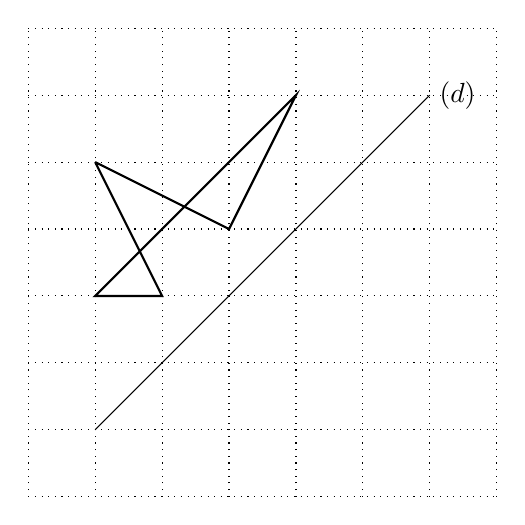
\begin{tikzpicture}[scale=0.85]
            \def\mypath{(-2,2) -- (-1,0) --(-2,0) -- (1,3)--(0,1)--(-2,2)}
            \draw [thick]\mypath ;
            \draw (-2,-2)--(3,3) node [right]{$(d)$} ;
            % \draw [cm={0,1,1,0,(0,0)}] \mypath;%Matrice de transformation inverse X et Y
            \draw [dotted](-3,-3) grid (4,4);
        \end{tikzpicture}
    \end{figure}
\end{minipage}
\hfill
\begin{minipage}[t]{0.45\textwidth}
    \exo{Représenter}{TracerSymAxQuadri2}
    
    \begin{figure}[H]
        \centering
        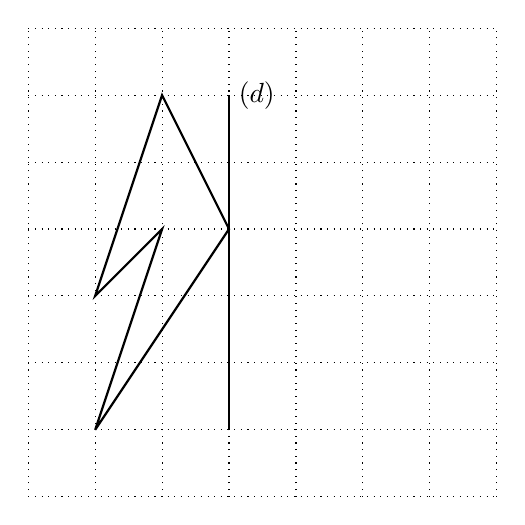
\begin{tikzpicture}[scale=0.85]
            \def\mypath{(-2,-2) -- (-1,1) --(-2,0) -- (-1,3)--(0,1)--(-2,-2)}
            \draw [thick]\mypath ;
            \draw (0,-2)--(0,3) node [right]{$(d)$} ;
            % \draw [cm={-1,0,0,1,(0,0)}] \mypath;%Matrice de transformation inverse X et Y
            \draw [dotted](-3,-3) grid (4,4);
        \end{tikzpicture}
    \end{figure}
\end{minipage}
\vspace{-1em}
\begin{minipage}[t]{0.45\textwidth}
    \exo{Représenter}{TracerSymAxQuadri3}
    
    \begin{figure}[H]
        \centering
        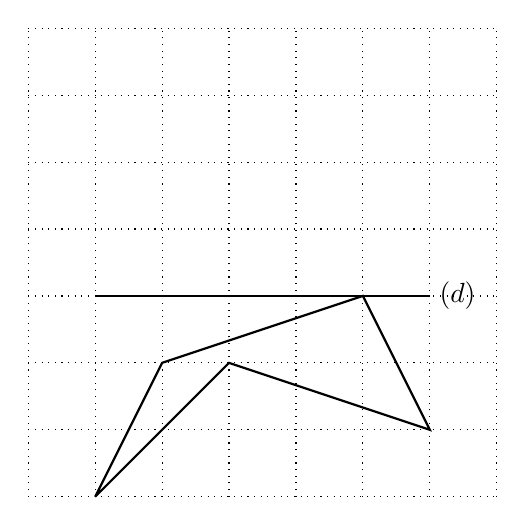
\begin{tikzpicture}[scale=0.85]
            \def\mypath{(-2,-3) -- (0,-1) --(3,-2) -- (2,0)--(-1,-1)--(-2,-3)}
            \draw [thick]\mypath ;
            \draw (-2,0)--(3,0) node [right]{$(d)$} ;
            % \draw [cm={1,0,0,-1,(0,0)}] \mypath;%Matrice de transformation inverse X et Y
            \draw [dotted](-3,-3) grid (4,4);
        \end{tikzpicture}
    \end{figure}
\end{minipage}
\hfill
\begin{minipage}[t]{0.45\textwidth}
    \exo{Représenter}{TracerSymAxQuadri4}
    
    \begin{figure}[H]
        \centering
        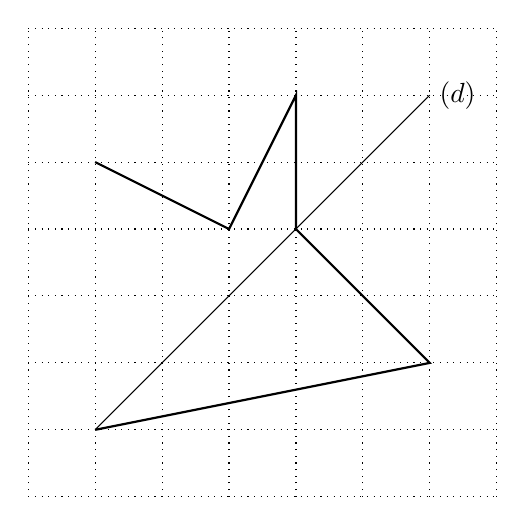
\begin{tikzpicture}[scale=0.85]
            \def\mypath{(-2,-2) -- (3,-1) --(1,1) -- (1,3)--(0,1)--(-2,2)}
            \draw [thick]\mypath ;
            \draw (-2,-2)--(3,3) node [right]{$(d)$} ;
            % \draw [cm={0,1,1,0,(0,0)}] \mypath;%Matrice de transformation inverse X et Y
            \draw [dotted](-3,-3) grid (4,4);
        \end{tikzpicture}
    \end{figure}
\end{minipage}

\vspace{2em}
\textbf{Pour les exercices \ref{TracerSymCentQuadri1} à \ref{TracerSymCentQuadri8} :} Tracer l'image de la figure suivante par la symétrie de centre $O$.
\vspace{-2em}

\begin{minipage}[t]{0.45\textwidth}
    \exo{Représenter}{TracerSymCentQuadri1}
    
    \begin{figure}[H]
        \centering
        \begin{tikzpicture}[scale=0.85]
            \tikzset{
                homothety at/.style args={#1 scaled by #2}{shift={($(#1)!#2!(0,0)$)},scale=#2},}
            \def\mypath{(-2,2) -- (-1,1) --(-2,0) -- (1,3)--(0,1)--(-2,2)}
            \draw [thick]\mypath ;
            \fill (0,0) coordinate (c) circle(2pt) node [above] {$O$};
            % \begin{scope}[homothety at=c scaled by -1]
            %     \draw \mypath;
            % \end{scope}
            \draw [dotted](-3,-3) grid (4,4);
        \end{tikzpicture}
    \end{figure}
\end{minipage}
\hfill
\begin{minipage}[t]{0.45\textwidth}
    \exo{Représenter}{TracerSymCentQuadri2}
    
    \begin{figure}[H]
        \centering
        \begin{tikzpicture}[scale=0.85]
            \tikzset{
                homothety at/.style args={#1 scaled by #2}{shift={($(#1)!#2!(0,0)$)},scale=#2},}
            \def\mypath{(-2,-2) -- (-1,1) --(-2,0) -- (-1,3)--(0,1)--(-2,-2)}
            \draw [thick]\mypath ;
            \fill (1,0) coordinate (c) circle(2pt) node [above] {$O$};
            % \begin{scope}[homothety at=c scaled by -1]
            %     \draw \mypath;
            % \end{scope}
            \draw [dotted](-3,-3) grid (4,4);
        \end{tikzpicture}
    \end{figure}
\end{minipage}

\begin{minipage}[t]{0.45\textwidth}
    \exo{Représenter}{TracerSymCentQuadri3}
    
    \begin{figure}[H]
        \centering
        \begin{tikzpicture}[scale=0.85]
            \tikzset{
                homothety at/.style args={#1 scaled by #2}{shift={($(#1)!#2!(0,0)$)},scale=#2},}
            \def\mypath{(-2,-2) -- (0,-1) --(3,-2) -- (2,0)--(-1,-1)--(-2,-2)}
            \draw [thick]\mypath ;
            \fill (0,0) coordinate (c) circle(2pt) node [above] {$O$};
            % \begin{scope}[homothety at=c scaled by -1]
            %     \draw \mypath;
            % \end{scope}
            \draw [dotted](-3,-3) grid (4,4);
        \end{tikzpicture}
    \end{figure}
\end{minipage}
\hfill
\begin{minipage}[t]{0.45\textwidth}
    \exo{Représenter}{TracerSymCentQuadri4}
    
    \begin{figure}[H]
        \centering
        \begin{tikzpicture}[scale=0.85]
            \tikzset{
                homothety at/.style args={#1 scaled by #2}{shift={($(#1)!#2!(0,0)$)},scale=#2},}
            \def\mypath{(-2,-2) -- (2,-2) --(0,2) -- (1,3)--(0,1)--(-2,2)}
            \draw [thick]\mypath ;
            \fill (0,1) coordinate (c) circle(2pt) node [above] {$O$};
            % \begin{scope}[homothety at=c scaled by -1]
            %     \draw \mypath;
            % \end{scope}
            \draw [dotted](-3,-3) grid (4,4);
        \end{tikzpicture}
    \end{figure}
\end{minipage}


\begin{minipage}[t]{0.45\textwidth}
    \exo{Représenter}{TracerSymCentQuadri5}
    
    \begin{figure}[H]
        \centering
        \begin{tikzpicture}[scale=0.85]
            \tikzset{
                homothety at/.style args={#1 scaled by #2}{shift={($(#1)!#2!(0,0)$)},scale=#2},}
            \def\mypath{(-2,2) -- (-1,1) --(-2,0) -- (1,3)--(0,1)--(-2,2)}
            \draw [thick]\mypath ;
            \fill (-1,0) coordinate (c) circle(2pt) node [above] {$O$};
            % \begin{scope}[homothety at=c scaled by -1]
            %     \draw[dashed] \mypath;
            % \end{scope}
            \draw [dotted](-3,-3) grid (4,4);
        \end{tikzpicture}
    \end{figure}
\end{minipage}
\hfill
\begin{minipage}[t]{0.45\textwidth}
    \exo{Représenter}{TracerSymCentQuadri6}
    
    \begin{figure}[H]
        \centering
        \begin{tikzpicture}[scale=0.85]
            \tikzset{
                homothety at/.style args={#1 scaled by #2}{shift={($(#1)!#2!(0,0)$)},scale=#2},}
            \def\mypath{(0,-3) -- (1,0) --(0,-1) -- (1,2)--(2,0)--(0,-3)}
            \draw [thick]\mypath ;
            \fill (1,0) coordinate (c) circle(2pt) node [above] {$O$};
            % \begin{scope}[homothety at=c scaled by -1]
            %     \draw[dashed] \mypath;
            % \end{scope}
            \draw [dotted](-3,-3) grid (4,4);
        \end{tikzpicture}
    \end{figure}
\end{minipage}

\begin{minipage}[t]{0.45\textwidth}
    \exo{Représenter}{TracerSymCentQuadri7}
    
    \begin{figure}[H]
        \centering
        \begin{tikzpicture}[scale=0.85]
            \tikzset{
                homothety at/.style args={#1 scaled by #2}{shift={($(#1)!#2!(0,0)$)},scale=#2},}
            \def\mypath{(-2,-2) -- (0,-1) --(3,-2) -- (2,0)--(-1,-1)--(-2,-2)}
            \draw [thick]\mypath ;
            \fill (1,1) coordinate (c) circle(2pt) node [above] {$O$};
            % \begin{scope}[homothety at=c scaled by -1]
            %     \draw[dashed] \mypath;
            % \end{scope}
            \draw [dotted](-3,-3) grid (4,4);
        \end{tikzpicture}
    \end{figure}
\end{minipage}
\hfill
\begin{minipage}[t]{0.45\textwidth}
    \exo{Représenter}{TracerSymCentQuadri8}
    
    \begin{figure}[H]
        \centering
        \begin{tikzpicture}[scale=0.85]
            \tikzset{
                homothety at/.style args={#1 scaled by #2}{shift={($(#1)!#2!(0,0)$)},scale=#2},}
            \def\mypath{(-2,-2) -- (2,-2) --(0,2) -- (1,3)--(0,1)--(-2,2)}
            \draw [thick]\mypath ;
            \fill (0,0) coordinate (c) circle(2pt) node [above] {$O$};
            % \begin{scope}[homothety at=c scaled by -1]
            %     \draw[dashed] \mypath;
            % \end{scope}
            \draw [dotted](-3,-3) grid (4,4);
        \end{tikzpicture}
    \end{figure}
\end{minipage}